% Fig 2 — Pipeline (schematic only; Methods/caption carry detail)
\documentclass[border=0pt,tikz]{standalone}
\makeatletter\@namedef{ver@sansmathfonts.sty}{2023/01/01}\makeatother
% Nature Portfolio / Scientific Data shared TikZ style for IRexp figures.
% Width: 183 mm double-column. Typography: Helvetica-class (phv).
\RequirePackage{tikz}
\RequirePackage{pgfplots}
\RequirePackage{xcolor}
\RequirePackage{helvet}
\IfFileExists{sansmathfonts.sty}{\RequirePackage{sansmathfonts}}{}
\renewcommand{\familydefault}{\sfdefault}
\pgfplotsset{compat=1.18}
\usetikzlibrary{
  arrows.meta,calc,positioning,fit,shapes.geometric,shapes.misc,
  backgrounds,shadows.blur,patterns,decorations.pathreplacing
}

% ---- Paul Tol / NMRexp-matched palette ----
\definecolor{nmrBlue}{HTML}{4A7EBB}
\definecolor{nmrBlueDark}{HTML}{2E5F8F}
\definecolor{nmrBlueLight}{HTML}{A8C8E8}
\definecolor{nmrPeach}{HTML}{E8B48C}
\definecolor{nmrNavy}{HTML}{1B3D5C}
\definecolor{nmrRed}{HTML}{C44E52}
\definecolor{nmrGreen}{HTML}{3D8B5E}
\definecolor{nmrOrange}{HTML}{D97B32}
\definecolor{ink}{HTML}{1A1A1A}
\definecolor{muted}{HTML}{7A7F85}
\definecolor{note}{HTML}{5C636A}
\definecolor{faint}{HTML}{E8EAEC}
\definecolor{ghost}{HTML}{C5C9CD}
\definecolor{tintBlue}{HTML}{EEF3F8}
\definecolor{tintGreen}{HTML}{EAF4EE}

\newcommand{\NatureFont}{\fontfamily{phv}\selectfont}
\newcommand{\PanelLabel}[1]{%
  {\NatureFont\bfseries\fontsize{8}{9.6}\selectfont #1}%
}
\newcommand{\FigBody}{\NatureFont\fontsize{7}{8.4}\selectfont}
\newcommand{\FigSmall}{\NatureFont\fontsize{5.5}{6.6}\selectfont}
\newcommand{\FigAxis}{\NatureFont\fontsize{7}{8.4}\selectfont}

\tikzset{
  nature arrow/.style={
    -{Latex[length=1.6mm,width=1.3mm]},
    line width=0.55pt, ink
  },
  nature arrow grey/.style={
    -{Latex[length=1.6mm,width=1.3mm]},
    line width=0.5pt, note
  },
  stage card/.style={
    draw=nmrBlueDark, line width=0.7pt, rounded corners=2.2pt,
    fill=white, inner sep=3pt, align=center, font=\FigBody
  },
  stage header/.style={
    fill=nmrBlueDark, text=white, font=\FigBody\bfseries,
    rounded corners=2.2pt, inner sep=2.5pt, align=center
  },
  soft card/.style={
    draw=ghost, line width=0.55pt, rounded corners=2.2pt,
    fill=white, inner sep=3.5pt, align=left, font=\FigBody
  },
}

\pgfplotsset{
  nature axis/.style={
    tick label style={font=\FigSmall, /pgf/number format/assume math mode},
    label style={font=\FigAxis\bfseries},
    title style={font=\FigBody\bfseries, color=ink},
    axis line style={ink, line width=0.5pt},
    tick style={ink, line width=0.45pt},
    major grid style={faint, line width=0.35pt},
    axis x line=bottom,
    axis y line=left,
    enlarge x limits=false,
    clip=false,
  },
  nature hbar/.style={
    nature axis,
    xbar,
    bar width=7pt,
    y=data,
    nodes near coords,
    every node near coord/.append style={
      font=\FigSmall, ink, anchor=west, /pgf/number format/fixed,
      /pgf/number format/1000 sep={,}
    },
    xtick=\empty,
    axis x line=none,
    y axis line style={ink, line width=0.55pt},
    ytick style={draw=none},
    y tick label style={font=\FigBody, ink, anchor=east},
    grid=major x,
    xmin=0,
  },
}

\usepackage[helvet]{sfmath}
\renewcommand{\familydefault}{\sfdefault}

\begin{document}\NatureFont
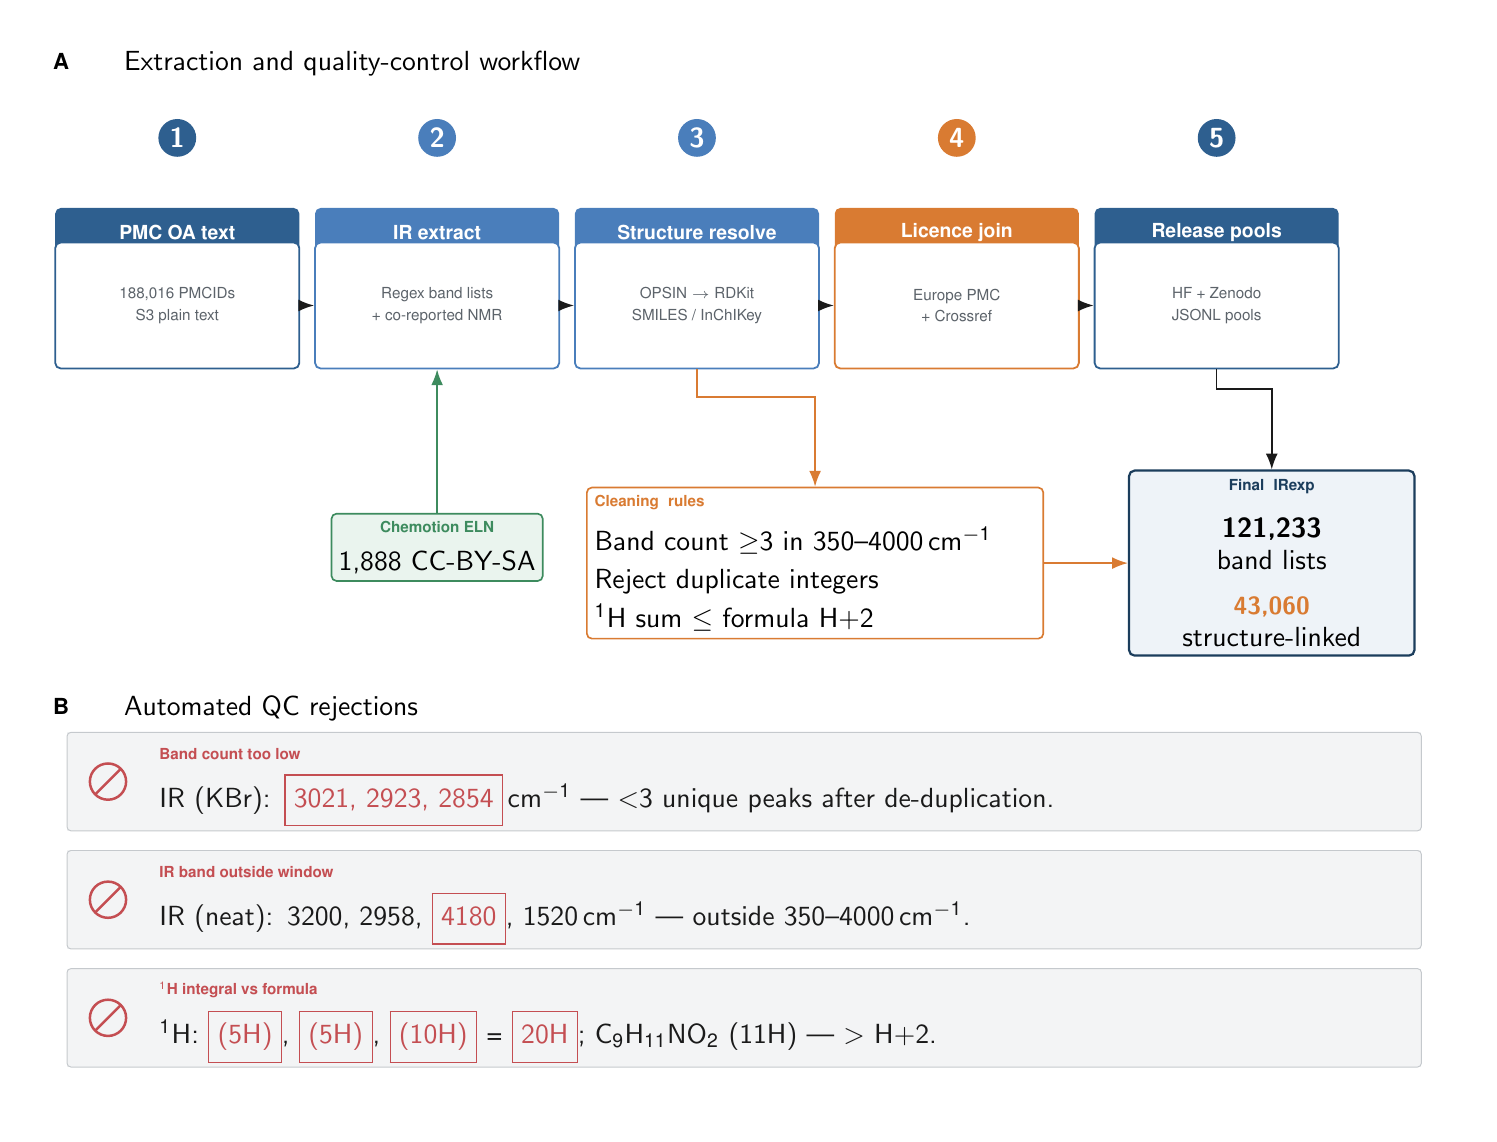
\begin{tikzpicture}[x=1mm,y=1mm,
  arr/.style={-{Latex[length=2.0mm,width=1.5mm]}, line width=0.6pt, ink},
  card/.style={
    draw=#1, line width=0.65pt, rounded corners=2pt, fill=white,
    minimum width=31mm, minimum height=16mm, align=center,
    font=\FigSmall, inner xsep=2.6pt, inner ysep=2.0pt
  },
  hdr/.style={
    fill=#1, text=white, font=\FigBody\bfseries, rounded corners=2pt,
    minimum width=31mm, minimum height=6.2mm, align=center, inner sep=1.1pt
  }]

\useasboundingbox (0,0) rectangle (183,138);

% ===== Panel A =====
\node[anchor=north west] at (2,136) {\PanelLabel{A}};
\node[anchor=west] at (11,133.5) {\FigTitle Extraction and quality-control workflow};

\def\yH{112}
\foreach \i/\x/\title/\col/\linea/\lineb in {%
  1/19/PMC OA text/nmrBlueDark/{188{,}016 PMCIDs}/{S3 plain text},%
  2/52/IR extract/nmrBlue/{Regex band lists}/{+ co-reported NMR},%
  3/85/Structure resolve/nmrBlue/{OPSIN $\to$ RDKit}/{SMILES / InChIKey},%
  4/118/Licence join/nmrOrange/{Europe PMC}/{+ Crossref},%
  5/151/Release pools/nmrBlueDark/{HF + Zenodo}/{JSONL pools}%
} {
  \node[circle, fill=\col, text=white, font=\FigTiny\bfseries,
        inner sep=0pt, minimum size=4.8mm] at (\x,{\yH+12.0}) {\i};
  \node[hdr=\col] (h\i) at (\x,\yH) {\title};
  \node[card=\col, below=0pt of h\i, yshift=2.0mm] (c\i)
    {{\FigTiny\color{note}\linea}\\[0.4ex]{\FigTiny\color{note}\lineb}};
}

\foreach \a/\b in {1/2,2/3,3/4,4/5} {
  \draw[arr] (c\a.east) -- (c\b.west);
}

\node[draw=nmrGreen, line width=0.6pt, rounded corners=1.8pt, fill=tintGreen,
      align=center, font=\FigTiny, inner sep=2.6pt] (chem) at (52,72)
  {{\FigSmall\bfseries\color{nmrGreen}Chemotion ELN}\\[0.4ex]1{,}888 CC-BY-SA};
\draw[arr,nmrGreen] (chem.north) -- (c2.south);

\node[draw=nmrOrange, line width=0.6pt, rounded corners=1.8pt, fill=white,
      align=left, font=\FigTiny, inner sep=2.8pt, text width=56mm] (clean) at (100,70)
  {{\FigSmall\bfseries\color{nmrOrange}Cleaning rules}\\[0.9ex]
   Band count $\ge$3 in 350--4000\,cm$^{-1}$\\[0.4ex]
   Reject duplicate integers\\[0.4ex]
   $^{1}$H sum $\le$ formula H+2};
\draw[arr,nmrOrange] (c3.south) -- ++(0,-3.5) -| (clean.north);

\node[draw=nmrNavy, line width=0.8pt, rounded corners=2pt, fill=tintBlue,
      align=center, font=\FigTiny, inner sep=3.2pt, text width=34mm] (fin) at (158,70)
  {{\FigSmall\bfseries\color{nmrNavy}Final IRexp}\\[1.1ex]
   {\fontsize{10}{12}\selectfont\bfseries 121{,}233}\\[-0.1ex]
   {\FigTiny band lists}\\[1.0ex]
   {\fontsize{9}{11}\selectfont\bfseries\color{nmrOrange}43{,}060}\\[-0.1ex]
   {\FigTiny structure-linked}};
\draw[arr] (c5.south) -- ++(0,-2.5) -| (fin.north);
\draw[arr,nmrOrange] (clean.east) -- (fin.west);

% ===== Panel B =====
\node[anchor=north west] at (2,54) {\PanelLabel{B}};
\node[anchor=west] at (11,51.5) {\FigTitle Automated QC rejections};

\newcommand{\rej}[3]{%
  \begin{scope}[shift={(5,#1)}]
    \fill[faint!50] (0,0) rectangle (172,12.5);
    \draw[ghost,line width=0.35pt,rounded corners=1.4pt] (0,0) rectangle (172,12.5);
    \draw[nmrRed,line width=0.9pt] (5.2,6.25) circle (2.3mm);
    \draw[nmrRed,line width=0.9pt] (3.6,4.65) -- (6.8,7.85);
    \node[anchor=west,font=\FigSmall\bfseries,nmrRed] at (10.5,9.8) {#2};
    \node[anchor=north west,align=left,text width=155mm,font=\FigTiny,ink]
      at (10.5,8.4) {#3};
  \end{scope}
}

\rej{36}{Band count too low}{%
  IR (KBr): {\color{nmrRed}\fbox{\strut 3021, 2923, 2854}}\,cm$^{-1}$
  --- $<$3 unique peaks after de-duplication.}
\rej{21}{IR band outside window}{%
  IR (neat): 3200, 2958, {\color{nmrRed}\fbox{\strut 4180}}, 1520\,cm$^{-1}$
  --- outside 350--4000\,cm$^{-1}$.}
\rej{6}{$^{1}$H integral vs formula}{%
  $^{1}$H: {\color{nmrRed}\fbox{\strut(5H)}}, {\color{nmrRed}\fbox{\strut(5H)}}, {\color{nmrRed}\fbox{\strut(10H)}}
  $=$ {\color{nmrRed}\fbox{\strut 20H}}; C$_9$H$_{11}$NO$_2$ (11H) --- $>$ H+2.}
\end{tikzpicture}
\end{document}
